% Ein Beispielkapitel
%

\chapter{Grafikeinbindung und Indexerstellung}

\section{Abschnitt mit verschiebbarer Tabelle und Grafik}

Zun�chst referenzieren wir die Abbildung \ref{fig:computer_architecture} (mit \verb|\ref{fig:computer_architecture}|). Grafiken k�nnen auch direkt mit Latex erzeugt werden, z.B. mit dem tikz Paket (Abbildung \ref{fig:tikz}). Das Buch \cite{Hager10} kann mit \verb|\cite{Hager10}| referenziert werden. Die Tabelle \ref{tab:vergleich} (Referenz erzeugt mit \verb|\ref{tab:vergleich}|) darf nat�rlich nicht fehlen. Fu�noten\footnote{Ich bin eine Fu�note} (erzeugt mit \verb|\footnote{Ich bin eine Fu�note}|) k�nnen ebenfalls verwendet werden. Und im Quelltext sieht ein Indexeintrag mit Ober- und Unterbegriff folgenderma�en aus: \index{Oberbegriff!Unterbegriff}\verb|\index{Oberbegriff!Unterbegriff}|.

\begin{figure} %[htbp] %hier k�nnen noch Positionierungsw�nsche angegeben werden
	\centering   % Alles weitere zentrieren
	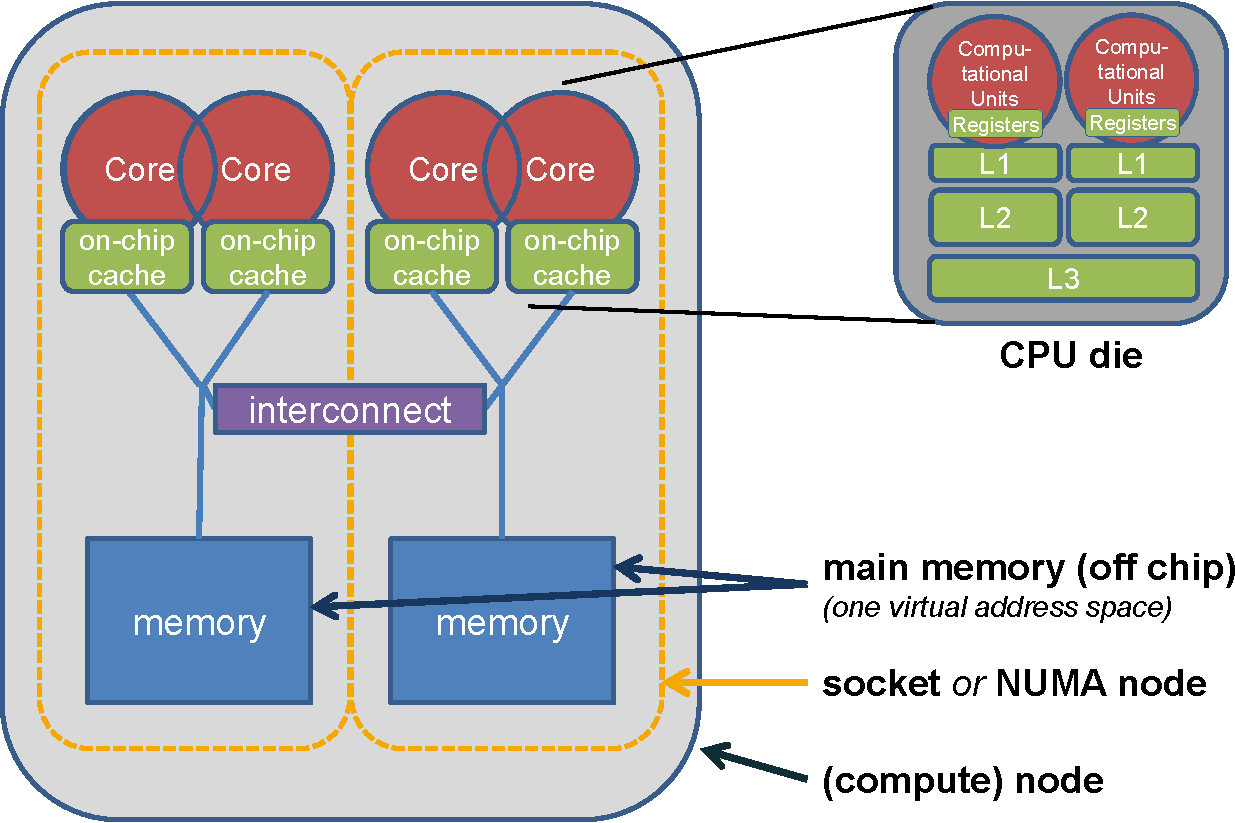
\includegraphics[width=13cm]{pictures/Computer}
	\caption{Parallele \index{Allgemein!Computer|(} Computerarchitektur (verschiebbare Grafik). Grafik erstellt von der HPC Gruppe des IT Centers.}
	\label{fig:computer_architecture}  %Reihenfolge ist wichtig! Immer erst \caption{} dann \label{}
\end{figure}


\begin{table} %[htbp] %hier k�nnen noch Positionierungsw�nsche angegeben werden
	\centering      % Alles weitere zentrieren
	\begin{tabular}{|c|c|c|c|} %Alle Spalten zentrieren, ansonsten 'r' oder 'l'
		\hline
		\textbf{Programming} & \textbf{Multi-}    & \textbf{Distributed} & \textbf{Accelerator} \\
		\textbf{Model}       & \textbf{processor} & \textbf{computer}    &                      \\
		\hline \hline
		OpenMP               & yes                & no                   & yes                  \\
		\hline
		MPI                  & yes                & yes                  & depends on            \\
		                     &                    &                      & accelerator           \\
		\hline
		OpenACC              & yes                & no 	                 & yes                   \\
		\hline
	\end{tabular}
	\caption{Einfacher Vergleich von OpenMP, MPI und OpenACC (verschiebbare Tabelle)}
	\label{tab:vergleich}  %Reihenfolge ist wichtig! Immer erst \caption{} dann \label{}
\end{table}

\tikzstyle{format} = [draw, thin, fill=blue!20]
\tikzstyle{medium} = [ellipse, draw, thin, fill=green!20, minimum height=2.5em]

\begin{figure}
	\begin{tikzpicture}[node distance=2cm, auto,>=latex', thick]
	% We need to set a bounding box first. Otherwise the diagram
	% will change position for each frame.
	%   \path[use as bounding box] (-5,0) rectangle (10,10);
	   \path[->] node[format](tex) {.tex file};
	   \path[->] node[format, right of=tex] at ($(tex.east)+(2.5em,0)$) (dvi) {.dvi file}
	     (tex) edge node {\TeX} (dvi);
	   \path[->] node[format, right of=dvi] at ($(dvi.east)+(2.5em,0)$) (ps) {.ps file}
	     node[medium, below of=dvi] at ($(dvi.south)-(0,2.5em)$)(screen) {screen}
	     (dvi) edge node {dvips} (ps)
	     edge node[swap] {xdvi} (screen);
	   \path[->] node[format, right of=ps] at ($(ps.east)+(2.5em,0)$) (pdf) {.pdf file}
	     node[medium, below of=ps] at ($(ps.south)-(0,2.5em)$) (print) {printer}
	     (ps) edge node {ps2pdf} (pdf)
	     edge node[swap] {gs} (screen)
	     edge (print);
	   \path[->] (pdf) edge (screen)
	     edge (print);
	   \path[->, draw] (tex) -- +(0,5) -| node[near start] {pdf\TeX} (pdf);   
	\end{tikzpicture}
	\caption{Latex Abbildung mit TIKZ \cite{Reble2013}}
	\label{fig:tikz}
\end{figure}


\section{Abschnitt mit ortsfester Tabelle und Grafik}

Eigentlich sollten ortsfeste Objekte nur sehr selten genutzt werden,
nichtsdestotrotz wird in diesem Abschnitt kurz gezeigt, wie man Grafiken und 
Tabellen ordentlich nummeriert und referenziert, obwohl sie nicht in eine 
\emph{figure} oder \emph{table} Umgebung eingebettet sind. Diese Art der
Einbindung erlaubt volle Kontrolle �ber die Platz\-ier\-ung der eingebundenen
Objekte.

\textbf{\emph{Hinweis:} Allerdings kann es passieren, dass die Floats hinter die
non-Floats verschoben werden und somit die Nummerierung "`falsch herum"'
vorgenommen wird.}

Hier werden wir einfach das RWTH-Logo \ref{fig:Logo} noch einmal genau
unter dieser Zeile einblenden:

\begin{nffigure} %Non-Floating Figure einbinden
	\centering
	
\includegraphics[width=6cm]{logo/rwth_itcenter_rgb.pdf}
	\caption{Das RWTH-Logo}
	\label{fig:Logo}  %Reihenfolge ist wichtig! Immer erst \caption{} dann \label{}
\end{nffigure}

Mit Tabellen funktioniert das ganz genau so (siehe \ref{tab:Testtabelle}):

\begin{nftable} %Non-Floating Table einbinden
	\centering
	\begin{tabular}{|c|c|c|}
		\hline
		Test1 & Test2 & Test3\\
		\hline
		Test4 & Test5 & Test6\\
		\hline
	\end{tabular}
	\caption{Eine ortsfeste Testtabelle}
	\label{tab:Testtabelle}  %Reihenfolge ist wichtig! Immer erst \caption{} dann \label{}
\end{nftable}
